\section[Cote 161-6 : le nombre d'or et les six axes de l'icosaèdre]{Cote 161-6 : le nombre d'or et les six axes de l'icosaèdre\protect\verifie[\leanblobmain]{Folder161_6}}\label{sec:161-6}

La cote 161-6, \emph{Graphes, icosaèdre [etc.] : notes manuscrites (s.d.)}, trente-trois pages que l'inventaire date \q{[à partir de 1973-vers 1977]}, réunit trois sujets sur des feuillets volants. Le premier est l'icosaèdre régulier. Une mise au net à l'encre le construit à partir de deux vecteurs unitaires orthogonaux $u$, $v$ et de l'angle $\theta = 2\pi/5$ (\lot{161-6}{1}{3}, \lot{161-6}{1}{4}), démontre que ses rotations sont au nombre de soixante (\lot{161-6}{1}{8}), puis le réduit à son graphe (\lot{161-6}{1}{10}). Deux pages calculent le nombre $2\cos(2\pi/5)$ dans l'anneau des racines cinquièmes de l'unité (\lot{161-6}{1}{14}, \lot{161-6}{1}{12}). La page~21 transporte l'icosaèdre sur une base quelconque, relativement à une forme quadratique (\lot{161-6}{2}{21}). On démontre ici ce qui, dans ces pages, est un calcul fini : la condition d'existence du triangle équilatéral, l'équation du nombre d'or et la fin du calcul de la page~6, l'équiangularité des six axes et le décompte des sommets, arêtes et faces. Les graphes sur les surfaces des pages~24 à~33 et le produit de frames des pages~12, 13 et~15 ne sont pas traités.

\noindent\emph{Le nombre d'or, pour commencer.} Le nombre d'or $\varphi = (1 + \sqrt5)/2$ est la racine positive de $t^2 = t + 1$ ; son inverse $\varphi^{-1} = \varphi - 1 = (\sqrt5 - 1)/2$ est racine de $t^2 + t - 1 = 0$. Il apparaît dans le pentagone régulier : le rapport de la diagonale au côté y vaut $\varphi$, et $2\cos(2\pi/5) = \varphi^{-1}$. Comme cinq faces de l'icosaèdre se rencontrent en chaque sommet, le pentagone des voisins d'un sommet fait entrer $\varphi$ dans toutes les mesures du solide. La mise au net ne le nomme jamais : il y figure sous la forme de l'équation $\eta^2 + \eta - 1 = 0$, avec $\eta = 2\cos(2\pi/5)$ ; la page~12 l'écrit $\gamma$, la page~21 $\gamma$ et $c$.

\noindent\emph{Conventions.} $E = \mathbb R^3$, de produit scalaire $B'(x, y) = x \cdot y$, de forme quadratique $Q(x) = x \cdot x$ et de forme polaire $B = 2B'$. Pour deux droites $D$, $D'$ engendrées par $x$ et $y$, on pose avec la page~12 $\cos'(D, D') = B(x, y)^2/(Q(x)Q(y)) - 2$, qui vaut $2\cos 2\alpha$ si $\alpha$ est l'angle des deux droites, défini au signe près. Les douze sommets sont pris, à similitude près, aux points
\[
(0, \pm 1, \pm\varphi), \qquad (\pm 1, \pm\varphi, 0), \qquad (\pm\varphi, 0, \pm 1),
\]
et les six axes sont les droites qui joignent deux sommets opposés, engendrées par $(0, 1, \pm\varphi)$, $(1, \pm\varphi, 0)$, $(\pm\varphi, 0, 1)$.

\subsection*{Le triangle équilatéral et l'angle $\alpha$ (pages 3 à 6)}

Sur la sphère unité, la page~3 trace le grand cercle issu de $u$ dans la direction $v$, $x(\alpha) = u\cos\alpha + v\sin\alpha$, et le même cercle tourné d'un angle $\theta$ autour de $u$. Les points $u$, $x$ et $x'$ obtenus à l'abscisse $\alpha$ forment un triangle isocèle, équilatéral si et seulement si
\[
(1')\qquad \cos\alpha = \frac{\cos\theta}{1 - \cos\theta}.
\]
La marge de la page~4 conclut qu'une solution existe pour $\theta \geq \pi/3$ (\lot{161-6}{1}{4}).

\begin{enonce}[Pages 3 et 4, forme corrigée par la lecture]
Pour $0 < \theta \leq \pi$, il existe $\alpha$ avec $0 < \alpha < \pi$ et $\cos\alpha = \cos\theta/(1 - \cos\theta)$ si et seulement si $\theta > \pi/3$. Pour $\theta = 2\pi/5$, on a $\cos(2\pi/5) = (\sqrt5 - 1)/4$, la solution est $\cos\alpha = 1/\sqrt5$, et $\cos 2\alpha = -3/5$.
\end{enonce}

\begin{proof}
Sur $[0, \pi]$, le cosinus est strictement décroissant, donc $\cos\theta < 1$ et $1 - \cos\theta > 0$. Si $\alpha$ existe, $\cos\alpha < 1$, d'où $\cos\theta < 1 - \cos\theta$, soit $\cos\theta < 1/2 = \cos(\pi/3)$ et $\theta > \pi/3$. Réciproquement, si $\theta > \pi/3$, alors $\cos\theta < 1/2$ et le quotient $q = \cos\theta/(1 - \cos\theta)$ est $< 1$ ; comme $\cos\theta \geq -1$, il est $\geq -1/2 > -1$. On prend $\alpha = \arccos q$, qui est dans $]0, \pi[$. Pour $\theta = 2\pi/5$, $\cos(2\pi/5) = 2\cos^2(\pi/5) - 1$ avec $\cos(\pi/5) = (1 + \sqrt5)/4$, ce qui donne $(\sqrt5 - 1)/4$ ; alors $q = (\sqrt5 - 1)/(5 - \sqrt5) = 1/\sqrt5$, car $(\sqrt5 - 1)\sqrt5 = 5 - \sqrt5$. Enfin $2/5 - 1 = -3/5$.
\end{proof}

\noindent En Lean : \texttt{exists\_alpha\_iff}, \texttt{cos\_two\_pi\_div\_five}, \texttt{cos\_alpha} et \texttt{cos\_two\_alpha}. L'inégalité doit être stricte : pour $\theta = \pi/3$, $q = 1$ et la seule solution est $\alpha = 0$, où le triangle se réduit à un point. C'est la correction que porte la lecture.

\begin{figure}[htbp]
\centering
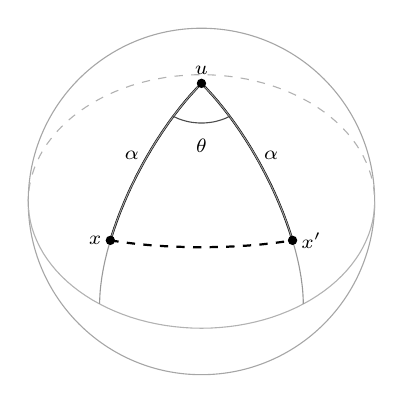
\begin{tikzpicture}[pt/.style={circle, fill, inner sep=1.2pt}, lab/.style={font=\scriptsize, inner sep=1pt}]
\draw[black!35] (0,0) circle (2.2);
\draw[black!30] (-1.293,-1.302) -- (-1.198,-1.350) -- (-1.100,-1.394) -- (-0.999,-1.434) -- (-0.895,-1.471) -- (-0.788,-1.503) -- (-0.680,-1.531) -- (-0.569,-1.555) -- (-0.457,-1.575) -- (-0.344,-1.590) -- (-0.230,-1.601) -- (-0.115,-1.608) -- (0.000,-1.610) -- (0.115,-1.608) -- (0.230,-1.601) -- (0.344,-1.590) -- (0.457,-1.575) -- (0.569,-1.555) -- (0.680,-1.531) -- (0.788,-1.503) -- (0.895,-1.471) -- (0.999,-1.434) -- (1.100,-1.394) -- (1.198,-1.350) -- (1.293,-1.302) -- (1.385,-1.251) -- (1.472,-1.196) -- (1.556,-1.138) -- (1.635,-1.077) -- (1.710,-1.013) -- (1.780,-0.946) -- (1.845,-0.877) -- (1.905,-0.805) -- (1.960,-0.731) -- (2.010,-0.655) -- (2.054,-0.577) -- (2.092,-0.497) -- (2.125,-0.417) -- (2.152,-0.335) -- (2.173,-0.252) -- (2.188,-0.168) -- (2.197,-0.084) -- (2.200,0.000);
\draw[black!30, dashed] (2.197,0.084) -- (2.188,0.168) -- (2.173,0.252) -- (2.152,0.335) -- (2.125,0.417) -- (2.092,0.497) -- (2.054,0.577) -- (2.010,0.655) -- (1.960,0.731) -- (1.905,0.805) -- (1.845,0.877) -- (1.780,0.946) -- (1.710,1.013) -- (1.635,1.077) -- (1.556,1.138) -- (1.472,1.196) -- (1.385,1.251) -- (1.293,1.302) -- (1.198,1.350) -- (1.100,1.394) -- (0.999,1.434) -- (0.895,1.471) -- (0.788,1.503) -- (0.680,1.531) -- (0.569,1.555) -- (0.457,1.575) -- (0.344,1.590) -- (0.230,1.601) -- (0.115,1.608) -- (0.000,1.610) -- (-0.115,1.608) -- (-0.230,1.601) -- (-0.344,1.590) -- (-0.457,1.575) -- (-0.569,1.555) -- (-0.680,1.531) -- (-0.788,1.503) -- (-0.895,1.471) -- (-0.999,1.434) -- (-1.100,1.394) -- (-1.198,1.350) -- (-1.293,1.302) -- (-1.385,1.251) -- (-1.472,1.196) -- (-1.556,1.138) -- (-1.635,1.077) -- (-1.710,1.013) -- (-1.780,0.946) -- (-1.845,0.877) -- (-1.905,0.805) -- (-1.960,0.731) -- (-2.010,0.655) -- (-2.054,0.577) -- (-2.092,0.497) -- (-2.125,0.417) -- (-2.152,0.335) -- (-2.173,0.252) -- (-2.188,0.168) -- (-2.197,0.084) -- (-2.200,0.000);
\draw[black!30] (-2.197,-0.084) -- (-2.188,-0.168) -- (-2.173,-0.252) -- (-2.152,-0.335) -- (-2.125,-0.417) -- (-2.092,-0.497) -- (-2.054,-0.577) -- (-2.010,-0.655) -- (-1.960,-0.731) -- (-1.905,-0.805) -- (-1.845,-0.877) -- (-1.780,-0.946) -- (-1.710,-1.013) -- (-1.635,-1.077) -- (-1.556,-1.138) -- (-1.472,-1.196) -- (-1.385,-1.251) -- (-1.293,-1.302);
\draw[thick] (0.000,1.500) -- (-0.024,1.475) -- (-0.048,1.451) -- (-0.072,1.425) -- (-0.095,1.399) -- (-0.119,1.373) -- (-0.143,1.347) -- (-0.167,1.319) -- (-0.190,1.292) -- (-0.214,1.264) -- (-0.237,1.235) -- (-0.261,1.206) -- (-0.284,1.177) -- (-0.307,1.147) -- (-0.330,1.117) -- (-0.353,1.087) -- (-0.376,1.056) -- (-0.399,1.025) -- (-0.422,0.993) -- (-0.444,0.961) -- (-0.466,0.929) -- (-0.489,0.896) -- (-0.511,0.863) -- (-0.532,0.830) -- (-0.554,0.797) -- (-0.576,0.763) -- (-0.597,0.729) -- (-0.618,0.695) -- (-0.639,0.661) -- (-0.659,0.626) -- (-0.680,0.591) -- (-0.700,0.556) -- (-0.720,0.521) -- (-0.740,0.485) -- (-0.759,0.450) -- (-0.778,0.414) -- (-0.797,0.378) -- (-0.816,0.342) -- (-0.834,0.306) -- (-0.852,0.269) -- (-0.870,0.233) -- (-0.888,0.197) -- (-0.905,0.160) -- (-0.922,0.124) -- (-0.938,0.087) -- (-0.955,0.050) -- (-0.970,0.014) -- (-0.986,-0.023) -- (-1.001,-0.060) -- (-1.016,-0.096) -- (-1.031,-0.133) -- (-1.045,-0.169) -- (-1.059,-0.206) -- (-1.072,-0.242) -- (-1.086,-0.279) -- (-1.098,-0.315) -- (-1.111,-0.351) -- (-1.123,-0.387) -- (-1.134,-0.423) -- (-1.146,-0.459) -- (-1.157,-0.494);
\draw[thick] (0.000,1.500) -- (0.024,1.475) -- (0.048,1.451) -- (0.072,1.425) -- (0.095,1.399) -- (0.119,1.373) -- (0.143,1.347) -- (0.167,1.319) -- (0.190,1.292) -- (0.214,1.264) -- (0.237,1.235) -- (0.261,1.206) -- (0.284,1.177) -- (0.307,1.147) -- (0.330,1.117) -- (0.353,1.087) -- (0.376,1.056) -- (0.399,1.025) -- (0.422,0.993) -- (0.444,0.961) -- (0.466,0.929) -- (0.489,0.896) -- (0.511,0.863) -- (0.532,0.830) -- (0.554,0.797) -- (0.576,0.763) -- (0.597,0.729) -- (0.618,0.695) -- (0.639,0.661) -- (0.659,0.626) -- (0.680,0.591) -- (0.700,0.556) -- (0.720,0.521) -- (0.740,0.485) -- (0.759,0.450) -- (0.778,0.414) -- (0.797,0.378) -- (0.816,0.342) -- (0.834,0.306) -- (0.852,0.269) -- (0.870,0.233) -- (0.888,0.197) -- (0.905,0.160) -- (0.922,0.124) -- (0.938,0.087) -- (0.955,0.050) -- (0.970,0.014) -- (0.986,-0.023) -- (1.001,-0.060) -- (1.016,-0.096) -- (1.031,-0.133) -- (1.045,-0.169) -- (1.059,-0.206) -- (1.072,-0.242) -- (1.086,-0.279) -- (1.098,-0.315) -- (1.111,-0.351) -- (1.123,-0.387) -- (1.134,-0.423) -- (1.146,-0.459) -- (1.157,-0.494);
\draw[thick, dashed] (-1.157,-0.494) -- (-1.122,-0.500) -- (-1.087,-0.505) -- (-1.051,-0.510) -- (-1.015,-0.515) -- (-0.979,-0.520) -- (-0.943,-0.525) -- (-0.906,-0.529) -- (-0.869,-0.534) -- (-0.831,-0.538) -- (-0.794,-0.542) -- (-0.756,-0.546) -- (-0.717,-0.549) -- (-0.679,-0.553) -- (-0.640,-0.556) -- (-0.601,-0.559) -- (-0.562,-0.562) -- (-0.523,-0.564) -- (-0.483,-0.567) -- (-0.443,-0.569) -- (-0.404,-0.571) -- (-0.364,-0.573) -- (-0.324,-0.575) -- (-0.283,-0.576) -- (-0.243,-0.577) -- (-0.203,-0.578) -- (-0.162,-0.579) -- (-0.122,-0.580) -- (-0.081,-0.581) -- (-0.041,-0.581) -- (0.000,-0.581) -- (0.041,-0.581) -- (0.081,-0.581) -- (0.122,-0.580) -- (0.162,-0.579) -- (0.203,-0.578) -- (0.243,-0.577) -- (0.283,-0.576) -- (0.324,-0.575) -- (0.364,-0.573) -- (0.404,-0.571) -- (0.443,-0.569) -- (0.483,-0.567) -- (0.523,-0.564) -- (0.562,-0.562) -- (0.601,-0.559) -- (0.640,-0.556) -- (0.679,-0.553) -- (0.717,-0.549) -- (0.756,-0.546) -- (0.794,-0.542) -- (0.831,-0.538) -- (0.869,-0.534) -- (0.906,-0.529) -- (0.943,-0.525) -- (0.979,-0.520) -- (1.015,-0.515) -- (1.051,-0.510) -- (1.087,-0.505) -- (1.122,-0.500) -- (1.157,-0.494);
\draw[black!40] (0.000,1.500) -- (-0.034,1.465) -- (-0.068,1.429) -- (-0.101,1.393) -- (-0.135,1.355) -- (-0.169,1.317) -- (-0.202,1.277) -- (-0.236,1.237) -- (-0.269,1.196) -- (-0.302,1.154) -- (-0.335,1.111) -- (-0.367,1.068) -- (-0.400,1.024) -- (-0.432,0.979) -- (-0.463,0.933) -- (-0.495,0.887) -- (-0.526,0.840) -- (-0.557,0.793) -- (-0.587,0.745) -- (-0.617,0.696) -- (-0.647,0.648) -- (-0.676,0.598) -- (-0.704,0.548) -- (-0.732,0.498) -- (-0.760,0.448) -- (-0.787,0.397) -- (-0.814,0.346) -- (-0.840,0.295) -- (-0.865,0.243) -- (-0.890,0.191) -- (-0.914,0.140) -- (-0.938,0.088) -- (-0.961,0.036) -- (-0.983,-0.016) -- (-1.005,-0.068) -- (-1.026,-0.120) -- (-1.046,-0.172) -- (-1.066,-0.224) -- (-1.085,-0.275) -- (-1.103,-0.327) -- (-1.120,-0.378) -- (-1.136,-0.429) -- (-1.152,-0.480) -- (-1.167,-0.530) -- (-1.181,-0.580) -- (-1.195,-0.629) -- (-1.207,-0.678) -- (-1.219,-0.727) -- (-1.230,-0.775) -- (-1.240,-0.823) -- (-1.249,-0.870) -- (-1.257,-0.916) -- (-1.265,-0.962) -- (-1.271,-1.007) -- (-1.277,-1.052) -- (-1.282,-1.095) -- (-1.286,-1.138) -- (-1.289,-1.181) -- (-1.291,-1.222) -- (-1.293,-1.263) -- (-1.293,-1.302);
\draw[black!40] (0.000,1.500) -- (0.034,1.465) -- (0.068,1.429) -- (0.101,1.393) -- (0.135,1.355) -- (0.169,1.317) -- (0.202,1.277) -- (0.236,1.237) -- (0.269,1.196) -- (0.302,1.154) -- (0.335,1.111) -- (0.367,1.068) -- (0.400,1.024) -- (0.432,0.979) -- (0.463,0.933) -- (0.495,0.887) -- (0.526,0.840) -- (0.557,0.793) -- (0.587,0.745) -- (0.617,0.696) -- (0.647,0.648) -- (0.676,0.598) -- (0.704,0.548) -- (0.732,0.498) -- (0.760,0.448) -- (0.787,0.397) -- (0.814,0.346) -- (0.840,0.295) -- (0.865,0.243) -- (0.890,0.191) -- (0.914,0.140) -- (0.938,0.088) -- (0.961,0.036) -- (0.983,-0.016) -- (1.005,-0.068) -- (1.026,-0.120) -- (1.046,-0.172) -- (1.066,-0.224) -- (1.085,-0.275) -- (1.103,-0.327) -- (1.120,-0.378) -- (1.136,-0.429) -- (1.152,-0.480) -- (1.167,-0.530) -- (1.181,-0.580) -- (1.195,-0.629) -- (1.207,-0.678) -- (1.219,-0.727) -- (1.230,-0.775) -- (1.240,-0.823) -- (1.249,-0.870) -- (1.257,-0.916) -- (1.265,-0.962) -- (1.271,-1.007) -- (1.277,-1.052) -- (1.282,-1.095) -- (1.286,-1.138) -- (1.289,-1.181) -- (1.291,-1.222) -- (1.293,-1.263) -- (1.293,-1.302);
\node[pt] at (0.000,1.500) {}; \node[lab,above=2pt] at (0.000,1.500) {$u$};
\node[pt] at (-1.157,-0.494) {}; \node[lab,left=2pt] at (-1.157,-0.494) {$x$};
\node[pt] at (1.157,-0.494) {}; \node[lab,right=2pt] at (1.157,-0.494) {$x'$};
\draw[black!70] (-0.357,1.081) -- (-0.326,1.066) -- (-0.293,1.051) -- (-0.259,1.039) -- (-0.224,1.028) -- (-0.188,1.018) -- (-0.151,1.010) -- (-0.114,1.004) -- (-0.076,1.000) -- (-0.038,0.997) -- (0.000,0.996) -- (0.038,0.997) -- (0.076,1.000) -- (0.114,1.004) -- (0.151,1.010) -- (0.188,1.018) -- (0.224,1.028) -- (0.259,1.039) -- (0.293,1.051) -- (0.326,1.066) -- (0.357,1.081);
\node[lab] at (0.000,0.713) {$\theta$};
\node[lab,left=2pt] at (-0.680,0.591) {$\alpha$}; \node[lab,right=2pt] at (0.680,0.591) {$\alpha$};
\end{tikzpicture}
\caption{Le triangle isocèle de la page~3 sur la sphère unité, pour $\theta = 2\pi/5$ : deux grands cercles issus de $u$ font l'angle $\theta$, et $x$, $x'$ sont à la distance $\alpha$ de $u$. Le triangle est équilatéral si et seulement si le troisième côté, en tireté, a lui aussi la longueur $\alpha$, ce qui demande $\cos\alpha = \cos\theta/(1 - \cos\theta)$, donc $\theta > \pi/3$ ; ici $\cos\alpha = 1/\sqrt5$. Figure de l'édition ; Grothendieck trace ces deux arcs en marge de la page~3 (\lot{161-6}{1}{3}).}
\label{fig:161-6-triangle}
\end{figure}

Les douze points sont alors $\pm u$ et $\pm x_i$, $x_i = u\cos\alpha + v_i\sin\alpha$, les $v_i$ étant les cinq directions tangentes d'angles $i\theta$ (figure~\ref{fig:161-6-calotte}). La page~5 veut montrer que la rotation $r = R_{w,\alpha} \circ R_{u,-\theta/2}$ envoie la calotte de sommet $u$ sur la calotte de sommet $x_0$. La page~6 vérifie la première des six relations nécessaires et s'arrête sur la troisième (\lot{161-6}{1}{6}). La lecture achève le calcul. Les coordonnées selon $w$ concordent d'elles-mêmes, et les autres se ramènent, avec $c = \cos\alpha$, à deux identités :
\[
\text{(A)}\quad c\,\bigl(1 - \cos\tfrac{2\pi}{5}\bigr) = \cos\tfrac{2\pi}{5}, \qquad \text{(B)}\quad c\,\bigl(1 + \cos\tfrac{\pi}{5}\bigr) = \cos\tfrac{\pi}{5}.
\]

\begin{enonce}[Page 6, achevée par la lecture]
Pour $c = 1/\sqrt5$, les identités (A) et (B) sont vraies.
\end{enonce}

\begin{proof}
(A) est la relation (1$'$), $c = \cos\theta/(1 - \cos\theta)$, multipliée par $1 - \cos\theta$. Pour (B), $\cos(\pi/5) = (1 + \sqrt5)/4$, et l'identité s'écrit $(5 + \sqrt5)/(4\sqrt5) = (1 + \sqrt5)/4$, soit $5 + \sqrt5 = \sqrt5 + 5$.
\end{proof}

\noindent En Lean : \texttt{identity\_A} et \texttt{identity\_B}. La réduction des six relations à (A) et (B) est celle de la lecture ; elle n'est pas formalisée. C'est seulement à cet endroit que $\theta = 2\pi/5$ intervient : la page~5 note que la construction des calottes vaut pour tout $\theta = 2\pi/m$.

\begin{figure}[htbp]
\centering
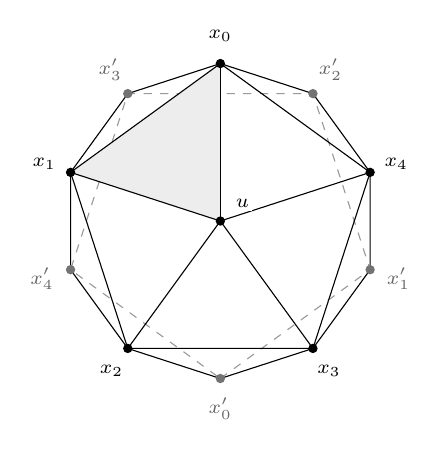
\begin{tikzpicture}[x=1cm, y=1cm, pt/.style={circle, fill, inner sep=1.2pt}, lab/.style={font=\scriptsize, inner sep=1pt}]
\foreach \i in {0,...,4} {
  \coordinate (x\i) at ({90+72*\i}:2);
  \coordinate (y\i) at ({270+72*\i}:2);
}
\coordinate (u) at (0,0);
\draw[black!40, dashed] (y0) -- (y1) -- (y2) -- (y3) -- (y4) -- cycle;
\fill[black!7] (u) -- (x0) -- (x1) -- cycle;
\draw (x0) -- (x1) -- (x2) -- (x3) -- (x4) -- cycle;
\foreach \i in {0,...,4} \draw (u) -- (x\i);
\draw (x0) -- (y3) -- (x1) -- (y4) -- (x2) -- (y0) -- (x3) -- (y1) -- (x4) -- (y2) -- cycle;
\foreach \i in {0,...,4} {
  \node[pt] at (x\i) {}; \node[lab] at ({90+72*\i}:2.35) {$x_{\i}$};
  \node[pt, black!55] at (y\i) {}; \node[lab, black!60] at ({270+72*\i}:2.38) {$x'_{\i}$};
}
\node[pt] at (u) {}; \node[lab, fill=white] at (0.28,0.22) {$u$};
\end{tikzpicture}
\caption{L'icosaèdre de la page~4 vu le long de l'axe $u$, $u' = -u$ caché derrière $u$. En noir, la calotte de sommet $u$, les cinq points $x_i$ en ordre circulaire, et les dix arêtes $\{x_i, x'_{i \pm 2}\}$ de la ceinture ; en tireté, le pentagone des $x'_i = -x_i$ de la face cachée. Grisé, le triangle icosaédral $\{u, x_0, x_1\}$. Figure de l'édition ; Grothendieck dessine l'icosaèdre en perspective en marge de la page~21 (figure~\ref{fig:161-6-axes}).}
\label{fig:161-6-calotte}
\end{figure}

\subsection*{L'équation du nombre d'or (pages 14 et 12)}

Les pages~14 et~12, à lire dans cet ordre, travaillent sur $\mathbb Z[\tfrac15]$, dans l'anneau $B = A[T]/(1 + T + T^2 + T^3 + T^4)$ des racines primitives cinquièmes de l'unité. Elles posent $\eta = \zeta + \zeta^{-1}$, $\eta' = \zeta^2 + \zeta^{-2}$, calculent la trace et la norme et en tirent \q{L'équation de $\gamma$ est donc $\gamma^2 + \gamma - 1 = 0$} (\lot{161-6}{1}{14}, \lot{161-6}{1}{12}).

\begin{enonce}[Pages 14 et 12]
Soit $A$ un anneau commutatif et $\zeta \in A$ tel que $1 + \zeta + \zeta^2 + \zeta^3 + \zeta^4 = 0$. Alors $\zeta^5 = 1$, et, pour $\eta = \zeta + \zeta^4$ et $\eta' = \zeta^2 + \zeta^3$,
\[
\eta + \eta' = -1, \qquad \eta\eta' = -1, \qquad \eta^2 + \eta - 1 = 0, \qquad \eta' = \eta^2 - 2, \qquad \eta = \eta'^2 - 2.
\]
Sur $\mathbb R$, avec $\zeta = e^{2i\pi/5}$, $\eta = 2\cos(2\pi/5) = \varphi^{-1} = (\sqrt5 - 1)/2$.
\end{enonce}

\begin{proof}
$\zeta^5 - 1 = (\zeta - 1)(1 + \zeta + \dots + \zeta^4) = 0$, donc $\zeta^{-1} = \zeta^4$ et $\zeta^{-2} = \zeta^3$. La trace est $\zeta + \zeta^2 + \zeta^3 + \zeta^4 = -1$. La norme est $\zeta^3 + \zeta^4 + \zeta^6 + \zeta^7 = \zeta^3 + \zeta^4 + \zeta + \zeta^2 = -1$. Un polynôme unitaire de degré~$2$ dont $\eta$ et $\eta'$ sont les racines est $t^2 - (\eta + \eta')t + \eta\eta' = t^2 + t - 1$. Enfin $\eta^2 = \zeta^2 + 2\zeta^5 + \zeta^8 = \eta' + 2$, et de même $\eta'^2 = \zeta^4 + 2 + \zeta = \eta + 2$. Sur $\mathbb R$, la valeur de $\cos(2\pi/5)$ vient de l'énoncé précédent, et $\varphi^{-1} = \varphi - 1$.
\end{proof}

\noindent En Lean : \texttt{trace\_norm}, \texttt{eta\_eq\_inv\_goldenRatio} et \texttt{eta\_golden}, avec le nombre d'or \texttt{Real.goldenRatio} de mathlib. L'énoncé ne demande aucune hypothèse sur l'anneau, ni que $5$ y soit inversible : c'est le passage à $\vartheta_5$, étale, qui l'exige. La lecture relie ce calcul à celui de la page~6, qu'il achève : (A) et (B) se ramènent à $\eta^2 + \eta - 1 = 0$. Les pages ne font pas ce lien.

\subsection*{Les six axes équiangulaires (page 21)}

La page~21 écrit \q{icosaèdre projectif --- icosaèdre} : ce qui se transporte sur une base, ce sont les six droites qui joignent les sommets opposés. La page calcule $\cos\alpha = \gamma/(2 - \gamma) = \frac15(2\gamma + 1) = 1/\sqrt5$, encadre $B(x, y)^2 = \frac45 Q(x)Q(y)$, puis $B'(x, y)^2 = \frac15 Q(x)Q(y)$ pour des générateurs $x$, $y$ de deux droites distinctes, et note $\cos'(D_i, D_j) = -6/5$ (\lot{161-6}{2}{21}).

\begin{encadre}
\begin{enonce}[Page 21, sur tout anneau où $t^2 = t + 1$]
Soit $R$ un anneau commutatif et $t \in R$ avec $t^2 = t + 1$. Les six vecteurs
\[
(0, 1, t),\ (0, 1, -t),\ (1, t, 0),\ (1, -t, 0),\ (t, 0, 1),\ (-t, 0, 1)
\]
ont tous $Q = t + 2$, et deux d'entre eux, distincts, vérifient $5\,B'(x_i, x_j)^2 = Q(x_i)Q(x_j)$. Sur $\mathbb R$, avec $t = \varphi$, les six axes de l'icosaèdre font donc deux à deux le même angle, de cosinus $\pm 1/\sqrt5$, et $\cos'(D_i, D_j) = -6/5$ pour $i \neq j$.
\end{enonce}
\end{encadre}

\begin{proof}
On a $B'(x_i, x_j) = \pm t$ ou $\pm(1 - t^2) = \mp t$, donc $B'(x_i, x_j)^2 = t^2$ dans tous les cas. Or $(t + 2)^2 = t^2 + 4t + 4 = 5t + 5 = 5t^2$. Sur $\mathbb R$, $Q > 0$, $B'^2/(QQ) = 1/5$ et $\cos' = 4/5 - 2 = -6/5$.
\end{proof}

\noindent En Lean : \texttt{axis\_norm}, \texttt{axes\_equiangular} et \texttt{cos'\_axes}. Sur un corps où $\gamma^2 + \gamma - 1 = 0$ et $5 \neq 0$, la page a raison : $2 - \gamma \neq 0$ et $\gamma/(2 - \gamma) = (2\gamma + 1)/5$ (\texttt{page21\_cos\_alpha}). L'énoncé est écrit sans division, ce que la forme $B'^2 = \frac15 QQ$ de la page masque. Il vaut donc sur $\mathbb Z[\varphi]$, et aussi en caractéristique~$5$, où $t = 3$ et $Q(x_i) = 0$ : les six axes y sont isotropes, comme dans la cote~70 (section~\ref{sec:70}). Six est le nombre maximal de droites équiangulaires dans un espace euclidien de dimension~$3$. L'énoncé n'en dit rien.

\begin{figure}[htbp]
\centering
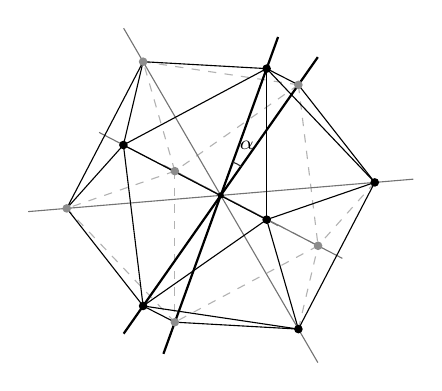
\begin{tikzpicture}[pt/.style={circle, fill, inner sep=1.1pt}, lab/.style={font=\scriptsize, inner sep=1pt}]
\draw[black!30, dashed] (0.986,1.404) -- (-0.583,0.308);
\draw[black!30, dashed] (0.986,1.404) -- (-0.986,1.698);
\draw[black!30, dashed] (0.986,1.404) -- (1.236,-0.640);
\draw[black!30, dashed] (1.956,0.165) -- (1.236,-0.640);
\draw[black!30, dashed] (-0.583,0.308) -- (-0.986,1.698);
\draw[black!30, dashed] (-0.583,0.308) -- (1.236,-0.640);
\draw[black!30, dashed] (-0.583,0.308) -- (-0.583,-1.610);
\draw[black!30, dashed] (-0.583,0.308) -- (-1.956,-0.165);
\draw[black!30, dashed] (0.986,-1.698) -- (1.236,-0.640);
\draw[black!30, dashed] (1.236,-0.640) -- (-0.583,-1.610);
\draw[black!30, dashed] (-0.583,-1.610) -- (-1.956,-0.165);
\draw[thick] (0.728,2.012) -- (-0.728,-2.012);
\draw[thick] (1.233,1.756) -- (-1.233,-1.756);
\draw[black!55] (2.445,0.206) -- (-2.445,-0.206);
\draw[black!55] (-0.728,0.385) -- (0.728,-0.385);
\draw[black!55] (1.233,-2.123) -- (-1.233,2.123);
\draw[black!55] (-1.545,0.800) -- (1.545,-0.800);
\draw (0.583,1.610) -- (0.986,1.404);
\draw (0.583,1.610) -- (1.956,0.165);
\draw (0.583,1.610) -- (-1.236,0.640);
\draw (0.583,1.610) -- (0.583,-0.308);
\draw (0.583,1.610) -- (-0.986,1.698);
\draw (0.986,1.404) -- (1.956,0.165);
\draw (1.956,0.165) -- (0.986,-1.698);
\draw (1.956,0.165) -- (0.583,-0.308);
\draw (0.986,-1.698) -- (0.583,-0.308);
\draw (0.986,-1.698) -- (-0.583,-1.610);
\draw (0.986,-1.698) -- (-0.986,-1.404);
\draw (-1.236,0.640) -- (0.583,-0.308);
\draw (-1.236,0.640) -- (-0.986,1.698);
\draw (-1.236,0.640) -- (-0.986,-1.404);
\draw (-1.236,0.640) -- (-1.956,-0.165);
\draw (0.583,-0.308) -- (-0.986,-1.404);
\draw (-0.986,1.698) -- (-1.956,-0.165);
\draw (-0.583,-1.610) -- (-0.986,-1.404);
\draw (-0.986,-1.404) -- (-1.956,-0.165);
\node[pt] at (0.583,1.610) {};
\node[pt, black!45] at (0.986,1.404) {};
\node[pt] at (1.956,0.165) {};
\node[pt, black!45] at (-0.583,0.308) {};
\node[pt] at (0.986,-1.698) {};
\node[pt] at (-1.236,0.640) {};
\node[pt] at (0.583,-0.308) {};
\node[pt, black!45] at (-0.986,1.698) {};
\node[pt, black!45] at (1.236,-0.640) {};
\node[pt, black!45] at (-0.583,-1.610) {};
\node[pt] at (-0.986,-1.404) {};
\node[pt, black!45] at (-1.956,-0.165) {};
\draw[black!80] (70.1:0.45) arc[start angle=70.1, end angle=54.9, radius=0.45];
\node[lab] at (62.5:0.72) {$\alpha$};
\node[pt, inner sep=0.8pt] at (0,0) {};
\end{tikzpicture}
\caption{Les six axes de l'icosaèdre, droites qui joignent les sommets opposés ; les sommets et les arêtes cachés sont en gris. Deux axes quelconques font le même angle $\alpha$, de cosinus $1/\sqrt5$ ; deux d'entre eux sont en gras. Figure de l'édition ; Grothendieck dessine l'icosaèdre en perspective en marge de la page~21 (\lot{161-6}{2}{21}).}
\label{fig:161-6-axes}
\end{figure}

En marge des énoncés a) à c), la page écrit \q{$c^2 + c - 1 = 0$} pour la constante $c = \cos'(D_i, D_j)$.

\begin{contrexemple}[Marge de la page 21]
La constante $c = \cos'(D_i, D_j) = -6/5$ n'est pas racine de $t^2 + t - 1$ : $c^2 + c - 1 = -19/25$.
\end{contrexemple}

\noindent En Lean : \texttt{margin\_false}. C'est $\eta = 2\cos(2\pi/5)$ qui vérifie l'équation du nombre d'or. Il sert à calculer $\cos\alpha$, mais il n'est pas l'invariant d'une paire d'axes. La lecture y voit la trace d'une autre définition de l'icosaèdre local, où la constante serait un nombre d'or, et que le calcul de la même page ne soutient pas.

La lecture propose une définition de l'icosaèdre relatif : six sous-modules de rang~$1$, localement facteurs directs, avec $B'(x_i, x_j)^2 = \frac15 Q(x_i)Q(x_j)$, sur une base où $2$ et~$5$ sont inversibles. Elle remarque que \q{localement} doit adjoindre $\sqrt5$.

\begin{enonce}[Énoncé de l'édition, d'après la lecture de la page 21]
Sur un corps $K$, si trois vecteurs $x_1$, $x_2$, $x_3$ vérifient $Q(x_i) \neq 0$ et $5\,B'(x_i, x_j)^2 = Q(x_i)Q(x_j)$ pour les trois paires, alors $5$ est un carré dans $K$. En particulier, il n'existe pas trois telles droites dans $\mathbb Q^3$.
\end{enonce}

\begin{proof}
Les hypothèses donnent $5 \neq 0$ et $b_{ij} = B'(x_i, x_j) \neq 0$. Le produit des trois relations donne $125\,(b_{12}b_{13}b_{23})^2 = (Q(x_1)Q(x_2)Q(x_3))^2$, et $r = Q(x_1)Q(x_2)Q(x_3)/(5\,b_{12}b_{13}b_{23})$ vérifie $r^2 = 5$. Sur $\mathbb Q$, $5$ n'est pas un carré, puisque $5$ n'est pas un carré d'entier.
\end{proof}

\noindent En Lean : \texttt{isSquare\_five\_of\_three\_lines} et \texttt{no\_three\_rat\_lines}. Les énoncés a), b) et c) de la page, existence locale, conjugaison locale par $\mathrm{SO}(Q)$ et groupe d'isotropie fini étale à fibres $\mathfrak A_5$, ne sont pas démontrés ici.

\subsection*{Sommets, arêtes, faces (pages 7 à 9)}

La page~7 définit les arêtes comme les paires de points de l'icosaèdre à distance minimale, et les faces comme les triples deux à deux reliés (\lot{161-6}{1}{7}).

\begin{enonce}[Pages 7 et 8]
Les douze sommets sont sur une même sphère. Entre deux sommets distincts, le carré de la distance prend trois valeurs, $4$, $6 + 2\sqrt5$ et $10 + 2\sqrt5$, la dernière pour deux sommets opposés. Chaque sommet a cinq voisins à la distance minimale ; il y a trente arêtes et vingt faces. L'application $x \mapsto -x$ permute les sommets et les arêtes, et son déterminant vaut $-1$.
\end{enonce}

\begin{proof}
On calcule dans $\mathbb Z[\sqrt5]$, en coordonnées doublées ($2\varphi = 1 + \sqrt5$), où l'égalité est décidable. Les cent quarante-quatre carrés de distances et les décomptes sont vérifiés par énumération dans le noyau de Lean (\texttt{decide}). En coordonnées doublées, les trois distances sont $16$, $24 + 8\sqrt5$ et $40 + 8\sqrt5$, c'est-à-dire quatre fois les valeurs de l'énoncé.
\end{proof}

\noindent En Lean : \texttt{vert\_norm}, \texttt{d2\_values}, \texttt{nbrs\_card}, \texttt{edges\_card}, \texttt{faces\_card}, \texttt{vert\_neg} et \texttt{det\_neg\_one}. Les pages~8 et~9 demandent de \q{montrer que \emph{tout} automorphisme du graphe est dans $\Gamma'$}, le groupe des soixante rotations. La lecture corrige en $\Gamma$, d'ordre $120$ : l'antipodie $-1$ est un automorphisme du graphe des arêtes, mais elle n'est pas une rotation. Que ce graphe ait exactement $120$ automorphismes est vérifié pour l'icosaèdre combinatoire de la cote~86 (section~\ref{sec:86}, \texttt{card\_aut}). L'identification des deux modèles n'est pas formalisée.

Ne sont pas démontrés ici : la transitivité simple de $\Gamma'$ sur les soixante arêtes orientées et $|\Gamma'| = 60$ (pages~7 et~8) ; les six relations de la page~6 au-delà de leur réduction à (A) et (B) ; l'isomorphisme $\Gamma' \simeq \mathfrak A_5$ par les cinq triples d'axes orthogonaux (page~18) ; les \q{systèmes cohérents} d'ordres circulaires de la page~10 ; les invariants de l'inversion sur $\mu_5^*$ et le quotient $\vartheta_n$ (page~14) ; les énoncés a) à c) de la page~21 ; la somme de frames des pages~15, 13 et~12 ; le produit de topos de la page~22 ; les plongements de graphes dans les surfaces (pages~24 à~30) et les graphes à groupe transitif (pages~32 et~33).
